\documentclass[a4paper,12pt]{article}

\usepackage[utf8]{inputenc}
\usepackage{lmodern}
\usepackage[margin=1cm]{geometry}
\usepackage{amsmath}
\usepackage{graphicx}
\usepackage{xcolor}
\usepackage{caption}
\usepackage{tikz}
\usetikzlibrary{arrows.meta,positioning,shapes.geometric,calc,fit}

\pagestyle{empty}

\begin{document}
\begin{figure}[p]
  \centering
  \makebox[\textwidth][c]{\resizebox{1.08\textwidth}{!}{%
  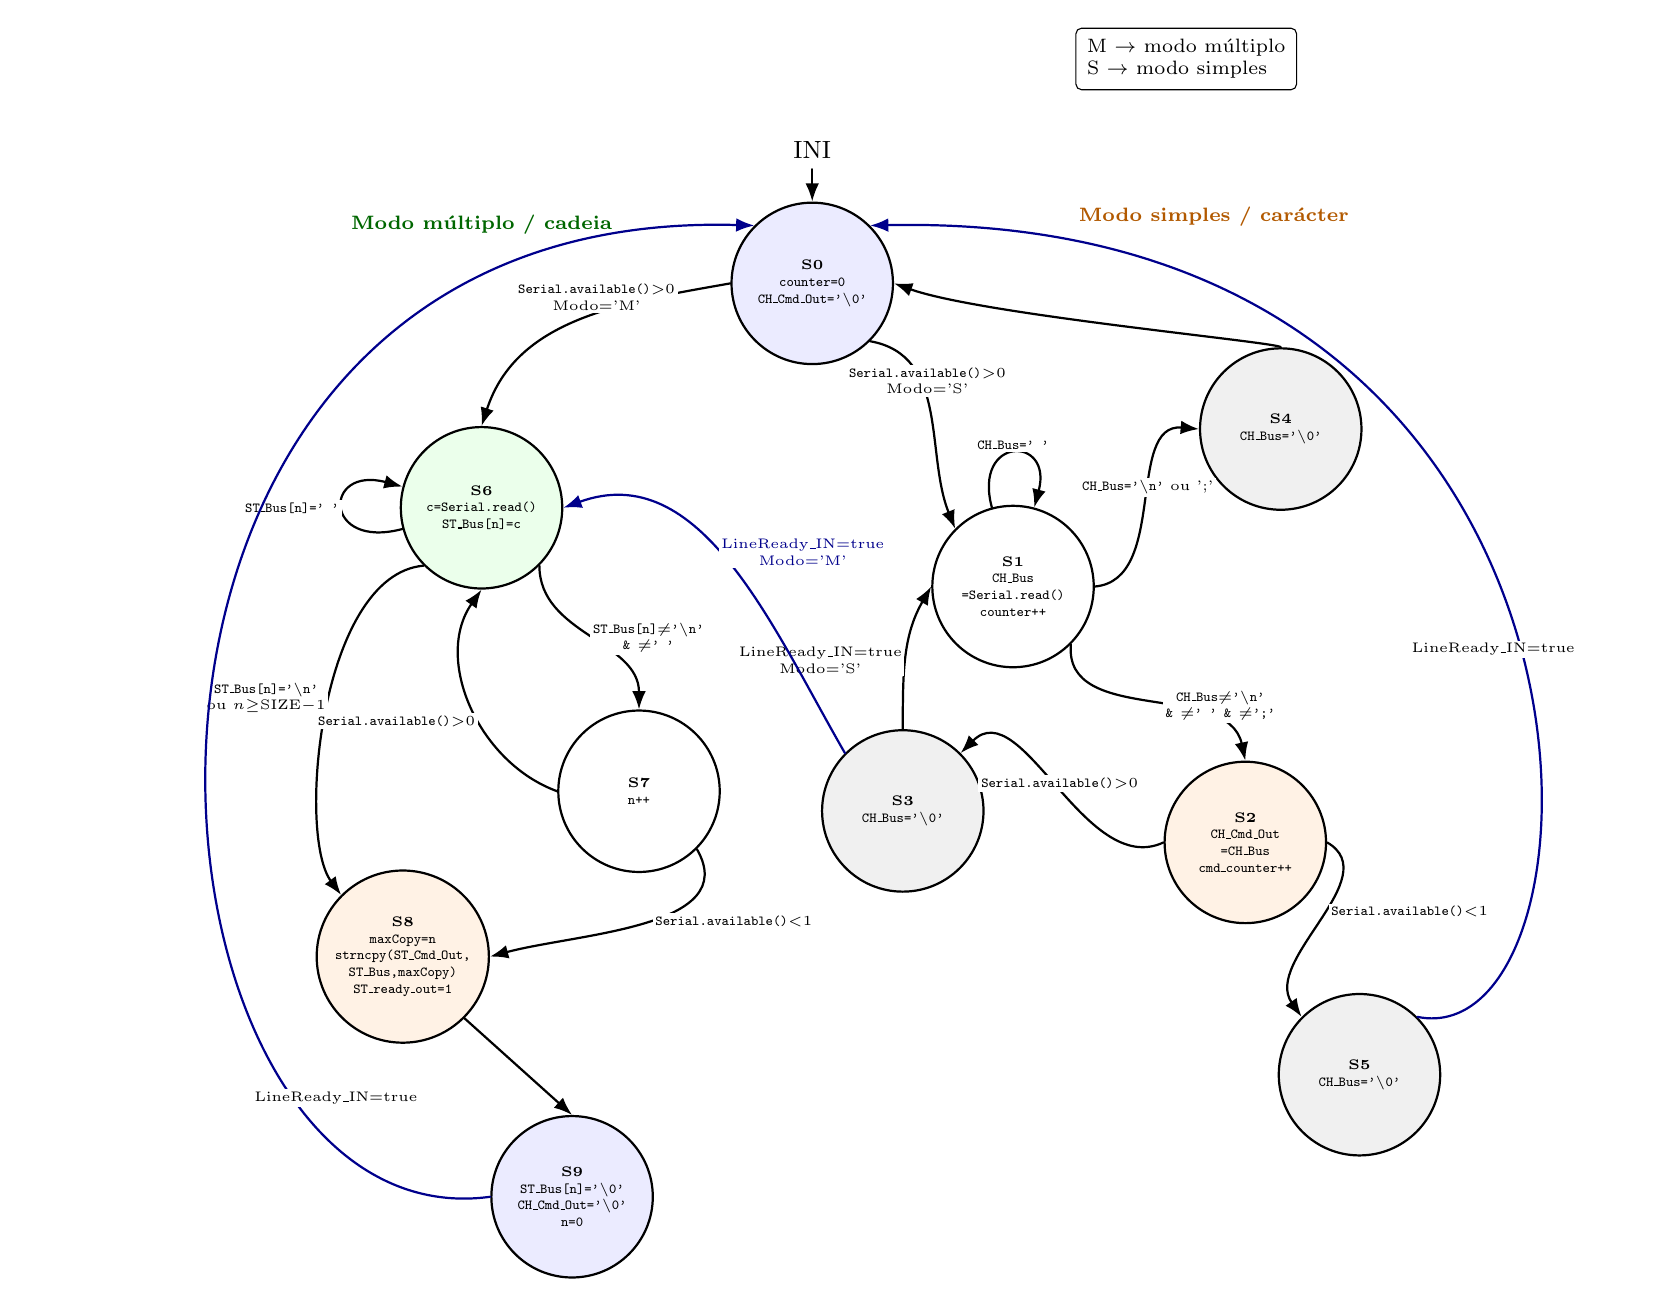
\begin{tikzpicture}[
    x=1cm,
    y=1cm,
    state/.style={draw, circle, align=center, minimum size=2.05cm, inner sep=2pt, font=\tiny, thick},
    smallstate/.style={state},
    widestate/.style={state},
    arrow/.style={-Latex, thick, line cap=round, line join=round},
    loopback/.style={-Latex, thick, blue!55!black, line cap=round, line join=round},
    softloop/.style={loopback, rounded corners=18pt},
    lab/.style={font=\tiny, align=center, fill=white, inner sep=1pt},
    >=Stealth
  ]
    \node[font=\scriptsize\bfseries, green!40!black] at (-4.20,14.55) {Modo múltiplo / cadeia};
    \node[font=\scriptsize\bfseries, orange!70!black] at (5.10,14.65) {Modo simples / carácter};
    \node[draw, rounded corners=2pt, align=left, font=\scriptsize, inner sep=4pt]
      at (4.75,16.65) {M $\to$ modo múltiplo\\S $\to$ modo simples};

    \node[state, fill=blue!8]      (r0) at (0,13.80)    {\textbf{S0}\\\texttt{counter=0}\\\texttt{CH\_Cmd\_Out='\textbackslash0'}};
    \node[smallstate, fill=green!8](r6) at (-4.20,10.95) {\textbf{S6}\\\texttt{c=Serial.read()}\\\texttt{ST\_Bus[n]=c}};
    \node[smallstate]              (r7) at (-2.20,7.35)  {\textbf{S7}\\\texttt{n++}};
    \node[widestate, fill=orange!10](r8) at (-5.20,5.25) {\textbf{S8}\\\texttt{maxCopy=n}\\\texttt{strncpy(ST\_Cmd\_Out,}\\\texttt{ST\_Bus,maxCopy)}\\\texttt{ST\_ready\_out=1}};
    \node[widestate, fill=blue!8]  (r9) at (-3.05,2.20)  {\textbf{S9}\\\texttt{ST\_Bus[n]='\textbackslash0'}\\\texttt{CH\_Cmd\_Out='\textbackslash0'}\\\texttt{n=0}};

    \node[smallstate]              (r1) at (2.55,9.95)  {\textbf{S1}\\\texttt{CH\_Bus}\\\texttt{=Serial.read()}\\\texttt{counter++}};
    \node[smallstate, fill=gray!12](r4) at (5.95,11.95)  {\textbf{S4}\\\texttt{CH\_Bus='\textbackslash0'}};
    \node[state, fill=orange!10]   (r2) at (5.50,6.70)   {\textbf{S2}\\\texttt{CH\_Cmd\_Out}\\\texttt{=CH\_Bus}\\\texttt{cmd\_counter++}};
    \node[smallstate, fill=gray!12](r3) at (1.15,7.10)   {\textbf{S3}\\\texttt{CH\_Bus='\textbackslash0'}};
    \node[smallstate, fill=gray!12](r5) at (6.95,3.75)   {\textbf{S5}\\\texttt{CH\_Bus='\textbackslash0'}};

    \draw[arrow] (0,15.25) node[above]{\small INI} -- (r0.north);

    \draw[arrow] (r0.west) to[out=190,in=72]
      node[lab, pos=0.43, above]{\texttt{Serial.available()}$>$0\\Modo$=$'M'} (r6.north);
    \draw[arrow] (r0.south east) to[out=350,in=112]
      node[lab, pos=0.43, above]{\texttt{Serial.available()}$>$0\\Modo$=$'S'} (r1.north west);

    \draw[arrow] (r6) to[loop left, min distance=1.05cm] node[lab, left]{\texttt{ST\_Bus[n]=' '}} (r6);
    \draw[arrow] (r6.south east) to[out=270,in=90]
      node[lab, right]{\texttt{ST\_Bus[n]$\neq$'\textbackslash n'}\\\texttt{\& $\neq$' '}} (r7.north);
    \draw[arrow] (r6.south west) .. controls (-6.25,10.10) and (-6.55,6.80) ..
      node[lab, pos=0.47, left]{\texttt{ST\_Bus[n]='\textbackslash n'}\\ou $n{\ge}$SIZE$-1$} (r8.north west);
    \draw[arrow] (r7.west) to[out=160,in=235]
      node[lab, pos=0.43, left]{\texttt{Serial.available()}$>$0} (r6.south);
    \draw[arrow] (r7.south east) to[out=300,in=15]
      node[lab, pos=0.47, right]{\texttt{Serial.available()}$<$1} (r8.east);
    \draw[arrow] (r8.south east) to (r9.north);
    \draw[loopback] (r9.west) .. controls (-8.85,1.55) and (-9.95,14.80) .. (r0.north west);
    \node[lab] at (-6.05,3.45) {LineReady\_IN$=$true};

    \draw[arrow] (r1) to[loop above, min distance=0.95cm] node[lab, above]{\texttt{CH\_Bus=' '}} (r1);
    \draw[arrow] (r1.east) to[out=5,in=175]
      node[lab, above, pos=0.52]{\texttt{CH\_Bus='\textbackslash n'} ou ';'} (r4.west);
    \draw[arrow] (r4.north) .. controls (5.95,13.05) and (2.15,13.40) .. (r0.east);
    \draw[arrow] (r1.south east) to[out=265,in=102]
      node[lab, right, pos=0.55]{\texttt{CH\_Bus$\neq$'\textbackslash n'}\\\texttt{\& $\neq$' ' \& $\neq$';'}} (r2.north);
    \draw[arrow] (r2.west) to[out=205,in=45]
      node[lab, pos=0.48, above]{\texttt{Serial.available()}$>$0} (r3.north east);
    \draw[arrow] (r2.east) to[out=330,in=125]
      node[lab, pos=0.45, right]{\texttt{Serial.available()}$<$1} (r5.north west);
    \draw[arrow] (r3.north) to[out=90,in=-120] node[lab, pos=0.46, left]{LineReady\_IN$=$true\\Modo$=$'S'} (r1.west);
    \draw[loopback] (r3.north west) to[out=120,in=20]  node[lab, pos=0.54, right]{LineReady\_IN$=$true\\Modo$=$'M'} (r6.east);
    \draw[loopback] (r5.north east) .. controls (10.30,3.95) and (10.65,14.75) .. (r0.north east);
    \node[lab] at (8.65,9.15) {LineReady\_IN$=$true};
  \end{tikzpicture}}}
  \caption{Esquema da FSM\_Serial\_Reader.}
  \label{fig:fsm-serial-reader}
\end{figure}

\end{document}
